\documentclass[10pt]{ltjsarticle}
\usepackage{layout,url}
\usepackage{graphicx}
\usepackage[haranoaji,deluxe]{luatexja-preset}
\usepackage{resume}
\pagestyle{empty}

\begin{document}
%\layout

\title{科学の健全な発展のために}

% 和文著者名
\author{
    72246424 仁戸田晃
}

% 和文概要
\begin{abstract}
科学の発展のために研究者としての自分がすべきだと考えていることを、自分の現在の研究と関連づけて述べる。
先に自分の研究内容である「デジタル学生証における発行者の秘匿と真正性検証の両立」について背景および前提知識
とともに述べ、その後、研究の持ちうる倫理的課題について論じる。
\end{abstract}

\maketitle
\thispagestyle{empty}

\section{研究の概要}
学生証の提示は、学生であることを確認するために広く用
いられている手法であるが、プライバシーの観点などから
学生証の発行者を秘匿してしまうと、学生証の真正性が担
保できなくなってしまう。そこで、検証可能な証明書である
Verifiable Credentials を用い、学校群を包括する群を導入
したアプローチをとることでこの問題を解決する。

\section{背景}

\subsection{学生であることの確認}
日常生活で、学生割引に適用や、学生限定のイベントな
ど、学生であることを確認したい・されたい場面は多く存在
する。その場合、現在用いられているのは主に学生証・在籍
証明証など、所属機関による所属証明の提示や、学校発行の
メールアドレスを用いた認証であり、本研究では学生証に着目する。
一般の学生証には、学校名、名前、学部、学籍
番号、顔写真、など様々な属性が記載されているが、学生証
を提示する人は、プライバシーの観点などから必要外の情報
を提供したくないことがあるということも想像できる。

\subsection{Verifiable Credentials}
学生証の一形態として、Verifiable Credential (以下、VCと呼称)を用いたも
のがある。Verifiable Credentials は、暗号学的な手法
で改ざん検知、および作成者が誰であるかの検証を可能にし
たCredential のこと、すなわち検証可能な証明書のことで
あり、ここでのCredentail とは発行者によって発行された、
対象となる主体に対する何らかの主張(Claim) の組と定義
される。Claimは、対象となる主体にまつわる「属性:値」のペアである。VC においては、発行者(Issuer)によって発行さ
れたVC を、保有者(Holder)が検証者(Verifier)に提示
するIHVモデルが取られている。なお、VC の示す主張の対象と
してのSubject と、VC のHolder は必ずしも同じである必
要はない。SubjectとHolderが異なる例として、子供に対して発行されたVCをその保護者が
保管する場合などが挙げられる。
Holder がVC をVerifier に提示する際、Holder
が、複数のVC を合わせ、VP が正しいことを示すProof
およびHolder であることを示すProof を含んで提示する
Verifiable Presentations (以下、VPと呼称) という形式をとることもで
きる。また、Holder はVC およびVP を任意のタイミング
で任意の属性を含んだ形で提示することもでき、任意の属性
の提示を可能にする技術として選択的開示が存在する。

\subsection{VCの一例}
VCを適用できる事例として、運転免許証が挙げられる。運転免許証において
先ほどのIHVモデルを適用すると、Issuerは各都道府県公安委員会であり、
Holderは運転免許証を交付され保持する人であり、Verifierは時と場合により異なりうる。
レンタカー会社が車を貸し出す時に運転免許証を確認する場合があるかもしれないし、アルコール等を購入する際に
年齢確認を行うために小売業者が運転免許証を確認する場合があるかもしれない。
また、選択的開示も可能である。Holderが年齢確認をされる場合、最低でも顔写真と生年月日の項目があれば必要十分であると
想定され、名前や住所などの情報は開示する必要はない。この場合、選択的開示を用いることで、顔写真と生年月日という
2つの属性が適切なIssuerによって主張され、改ざんされていないことをVerifierは暗号学的に検証することができる。

\begin{figure}[htbp]
    \begin{center}
        \includegraphics[width=6cm]{assets/IHVモデル.png}
        \caption{IHVモデル}
    \end{center}
\end{figure}

\begin{figure}[htbp]
    \begin{center}
        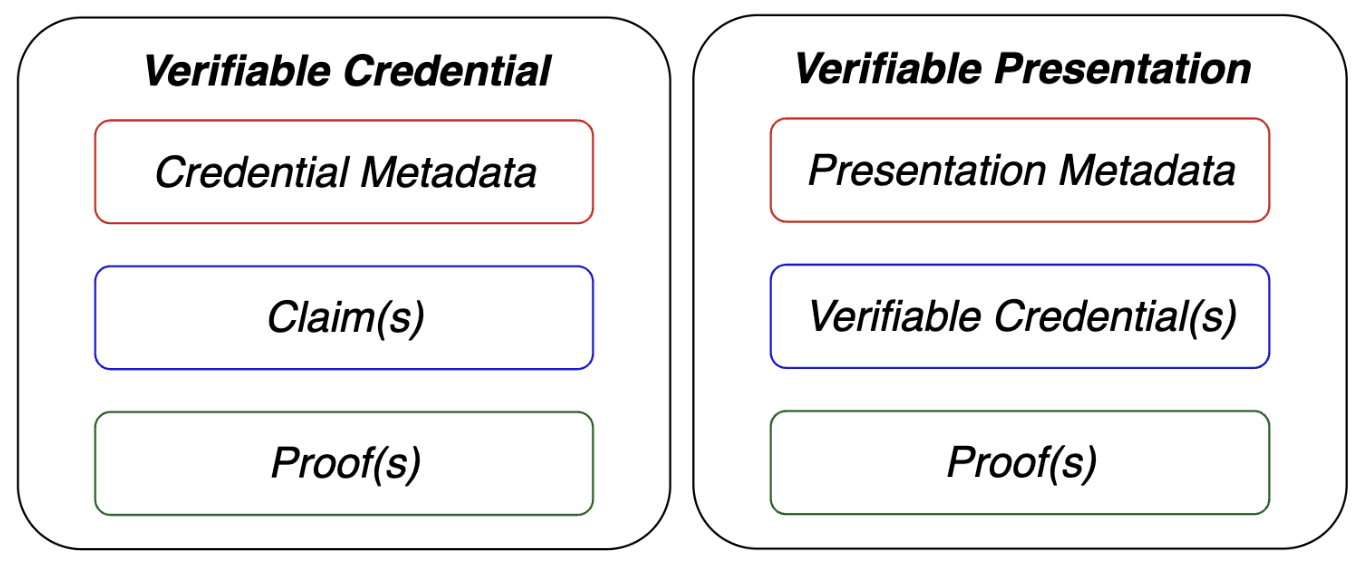
\includegraphics[width=6cm]{assets/VCとVP.png}
        \caption{VCおよびVP}
    \end{center}
\end{figure}

\begin{enumerate}
\item 番号付き箇条書き 
\item 番号付き箇条書き
\end{enumerate}

\begin{itemize}
\item 箇条書き
\item 箇条書き
\end{itemize}

%---------------------------------------------

\section{研究目的}

\subsection{hoge}
画像を図\ref{sample}に示す。

\begin{figure}[htbp]
    \begin{center}
        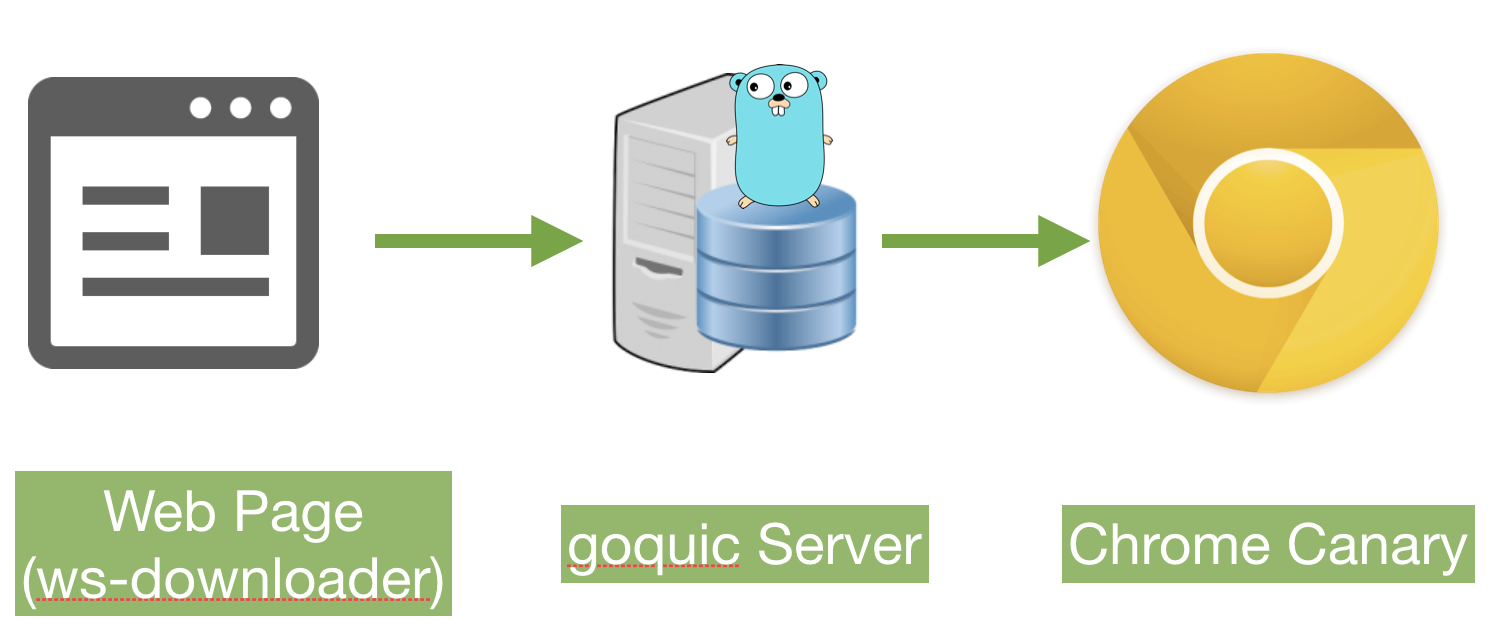
\includegraphics[width=6cm]{assets/figure1.png}
        \caption{画像の例}
        \label{sample}
    \end{center}
\end{figure}
 
\subsection{fuga}
fugafuga

\section{関連研究}

\section{提案手法}

\section{評価}

\section{考察}

\bibliographystyle{junsrt}
\bibliography{resume}

\end{document}
% end of file
